\documentclass{../lab_class}

\usepackage{fancyhdr}
\pagestyle{fancy}
\rhead{П.\,Ю. Смирнов, 687 гр.}
\lhead{Лабораторная работа № 3.122, МФТИ, осень 2017}

\newcommand{\ef}{\mathscr{E}}

\begin{document}

{\Large 3.122 -- Резонанс напряжений в последовательном контуре.}

\paragraph{Цель работы.}
Исследование резонанса напряжений в последовательном колебательном контуре с изменяемой ёмкостью, включающее получение амплитудно-частотных и фазово-частотных характеристик, а также определение основных параметров контура.

В работе используются: генератор сигналов, источник напряжения, нагруженный на последовательный колебательный контур с переменной ёмкостью, двулучевой осциллограф, цифровые вольтметры.

\paragraph{Теоретическая часть.}
В данной работе исследуется явление резонанса в <<обычной>> одномерной физической системе. Величиной, характеризующей систему, является заряд -- мы рассматриваем электрическую цепь, идеальный RLC-контур\footnote{В механике все аналогично. Резистор выражает трение в системе, катушка индуктивности -- инертность (массу), а конденсатор -- упругость. Вся математика совпадает.}. Вся математика рассматривамого процесса сводится к решению неоднородного дифференциального уравнения
\begin{equation}
	\ddot{q} + 2 \gamma \dot{q} + \omega_0^2 q = \ef_0 \sin \omega t,
\end{equation}
получаемого из того факта, что алгебраическая сумма падений напряжений вдоль всего контура равна внешней ЭДС.
Решать такое удобно над полем комплексных чисел; общее решение\footnote{$q$ здесь есть заряд конденсатора. В механике -- координата точки.} есть сумма некоторого частного решения и решения соотв. однородного уравнения: 
\begin{equation}
	q = \frac{\ef_0}{\omega^2_0 - \omega^2 + 2 i \omega \gamma} e^{i \omega t} + e^{-\gamma t} ( C_1 \cos{\omega_0 t} + C_2 \sin{\omega_0 t} );
\end{equation}
Второе слагаемое есть собственные колебания системы, они достаточно быстро затухают, в результате устанавливаются колебания на частоте внешней вынуждающей силы. Мы исследуем здесь поведение системы в установившемся режиме.

\begin{wrapfigure}[12]{r}{5cm}
	\centering
	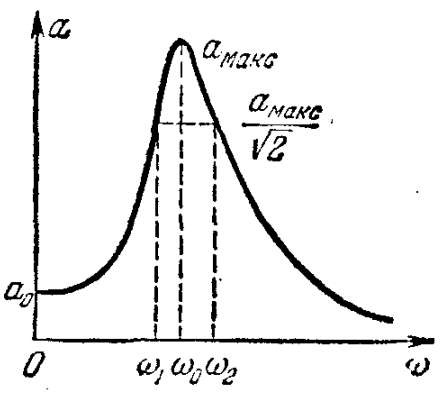
\includegraphics[width=4cm]{res_curve.png}
	\caption{Резонансная кривая}
\end{wrapfigure}

Физический смысл имеет лишь вещественная часть полученного решения. По формуле Эйлера получаем выражение для амплитуды и фазы установившегося колебания:
\begin{equation}\label{eq:ampl_phase}
\begin{aligned}
	&a = \frac{\ef_0}{\sqrt{(\omega_0^2 - \omega^2)^2 + 4 \omega^2 \gamma^2}}, \\
	&\tan{\delta} = \frac{2 \omega \gamma}{\omega_0^2 - \omega^2}.
\end{aligned}
\end{equation}

Максимум\footnote{Почему увеличение трения смещает максимум на АЧХ влево? Из тех же соображений, по которым частота свободных колебаний в системе с трением меньше, что ясно из механической аналогии -- при горизонтальном движении груза на пружине при наличии трения он остановится ( = отклонение достигнет максимума) раньше, чем при отсутствии трения. Впрочем, нужно обратить внимание на то, что частота свободных колебаний есть $\sqrt{\omega_0^2 - \gamma^2}$; максимум же АЧХ достигается при несколько меньшей частоте. Т.~о. неверно утверждение, что резонанс достигается при равенстве частоты свободных колебаний системы и частоты внешней силы.} амплитуды достигается при $\omega = \sqrt{\omega_0^2 - 2 \gamma^2}$. Практически важен случай, когда трение в системе мало, потому можно считать, что резонанс достигается при $\omega = \omega_0$; он и реализуется в нашей установке и рассматривается далее.

Важная характеристика систем с трением -- \emph{добротность}. Определим её следующим образом:
\begin{equation*}
	Q = 2 \pi \frac{W}{\Delta W},
\end{equation*}
где $W$ -- энергия запасенная в системе, а $\Delta W$ -- потери энергии (на трение) за один период. Итак, выше добротность = меньше потери на трение, меньше затухание колебаний. Смысл такого определения будет сейчас прояснен. Если мы хотим описать затухание в системе, то вместо энергии, вообще говоря, удобнее смотреть сразу на амплитуду. И действительно, вводят понятие \emph{логарифмического декремента затухания}:
\begin{equation*}
	\delta = \ln \frac{x(t)}{x(t+T)},
\end{equation*}
где $T$ -- период колебаний. Для свободных колебаний получаем $\delta = \gamma T$. Используя тот факт, что энергия пропорциональна квадрату амплитуды, и считая трение малым\footnote{В общем случае получается менее красивое выражение с экспонентой.}, мы легко получаем связь добротности и логарифмического декремента: $Q \approx \pi / \delta$. Если $\omega = 0$, то на систему действует постоянная сила, вызывающее статическое смещение $a_0 = \ef_0 / \omega_0$. Амплитуда при резонансе же $a_{\max} = \ef_0 / (2 \omega_0 \gamma)$; т.~о. получаем, что добротность $Q = a_{\max} / a_0$\footnote{Сивухин вообще определяет так добротность. Считаю, что это методологически неверно.}. Итак, выше добротность контура -- выше максимум резонансной кривой! В частности, если трения нет, то максимума нет в принципе, амплитуда может быть сколь угодно большой. 

Пусть $\omega_1$ и $\omega_2$ -- значения частоты, при которых энергия колебаний вдвое меньше энергии в максимуме. Снова используя известное отношение амплитуды и энергии и считая, что отклонение указанных частот от частоты резонанса на порядки меньше, чем, собственно, сами частоты, получаем приближенно
\begin{equation*}
	\Delta \omega \equiv \omega_2 - \omega_1 = 2 \gamma = Q / \omega_0.
\end{equation*}
Стало быть, добротность характеризует ещё и ширину резонансной кривой! Чем выше добротность, тем выше максимум АЧХ и уже ширина резонансной кривой. Это даёт нам и способ её экспериментального измерения -- ширина АЧХ при амплитуде $a_{\max}/\sqrt{2}$. Напоследок приведём выражение для добротности через параметры контура (легко получаемое из выражения связи добротности и логарифмического декремента): $Q = R \sqrt{\frac{L}{C}}$.

\begin{wrapfigure}[12]{r}{5cm}
	\centering
	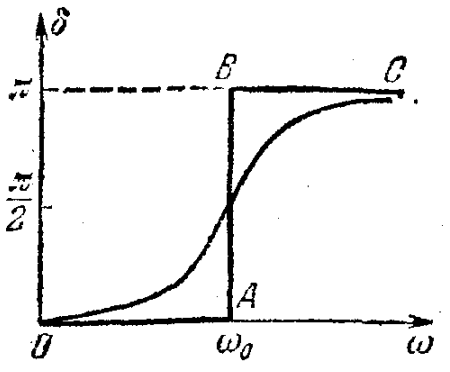
\includegraphics[width=4cm]{freq_curve.png}
	\caption{Фазово-частотная характеристика}
	\label{fig:phase_resp}
\end{wrapfigure}

Смещение (заряд) отстаёт по фазе от внешней силы на величину $\delta$. Как сразу видно из выражения \ref{eq:ampl_phase}, ФЧХ контура имеет вид, представленный на рис. \ref{fig:phase_resp}.

\end{document}